% This is a sample document using the University of Minnesota, Morris, Computer Science
% Senior Seminar modification of the ACM sig-alternate style. Much of this content is taken
% directly from the ACM sample document illustrating the use of the sig-alternate class. Certain
% parts that we never use have been removed to simplify the example, and a few additional
% components have been added.

% See https://github.com/UMM-CSci/Senior_seminar_templates for more info and to make
% suggestions and corrections.

\documentclass{sig-alternate}
\usepackage{color}
\usepackage[colorinlistoftodos]{todonotes}

%%%%% Uncomment the following line and comment out the previous one
%%%%% to remove all comments
%%%%% NOTE: comments still occupy a line even if invisible;
%%%%% Don't write them as a separate paragraph
%\newcommand{\mycomment}[1]{}

\begin{document}

% --- Author Metadata here ---
%%% REMEMBER TO CHANGE THE SEMESTER AND YEAR AS NEEDED
\conferenceinfo{UMM CSci Senior Seminar Conference, December 2015}{Morris, MN}

\title{Concurrent Compaction in JVM Garbage Collection}

\numberofauthors{1}

\author{
% The command \alignauthor (no curly braces needed) should
% precede each author name, affiliation/snail-mail address and
% e-mail address. Additionally, tag each line of
% affiliation/address with \affaddr, and tag the
% e-mail address with \email.
\alignauthor
Jacob P. Opdahl\\
	\affaddr{Division of Science and Mathematics}\\
	\affaddr{University of Minnesota, Morris}\\
	\affaddr{Morris, Minnesota, USA 56267}\\
	\email{opdah023@morris.umn.edu}
}

\maketitle
\begin{abstract}
This paper provides a brief overview of both garbage collection (GC) 
of memory and parallel processing. We then cover how 
parallel processing applies to GC. Specifically, these
concepts are focused within the context of the Java Virtual Machine (JVM).
With that foundation, we look at various algorithms that perform compaction of fragmented 
memory during the GC process. These algorithms are designed 
to run concurrent to the application running.
Such concurrently compacting GC behavior stems from a desire to reduce ``stop-the-world''
pauses of an application.
% The current paper format *only* allows inline comments using the todo
% macro. That's kind of a bummer, and it would be neat if someone figured
% out how to change the acmconf style to allow this. I suspect it isn't *hard*
% but there are quite a few details that have to be sorted out in synchrony.
\end{abstract}

\keywords{Garbage collection (GC), concurrency, compaction, Continuously Concurrent Compacting Collector (C4), Collie, Field Pinning Protocol (FPP)}


\section{Introduction}
\label{sec:introduction}

In programming languages, the allocation and deallocation
of memory for objects can be explicit or implicit. If done implicitly,
a language is said to have \emph{automatic memory management}. Some languages 
with automatic memory management are C\#, Java, and Python.
Use of automatic memory management is beneficial to programmers as it 
prevents them from worrying about the details of memory allocation and deallocation. 
However, programmers do not have control over how memory management occurs,
which can have negative impacts on application performance.

Memory for a program is not an unlimited resource. Automatic memory management
must remove unused objects from memory when appropriate.
Dead objects, or \emph{garbage}, are objects that can be shown
to be unreachable by the program~\cite{glossary:g}. Garbage should be deallocated to 
save space for new objects that will be created. The algorithm used to perform implicit
deallocation of garbage, by detecting and removing dead objects, 
is a \emph{garbage collector}.
We will focus on
garbage collection (GC) performed within Java Virtual Machines 
(JVMs), software processes that run programs written in Java and other languages 
on computing systems~\cite{Lindblom:2011}.

GC is not without cost.
Just like the application, GC requires processing resources to run. When using a single processor, 
we get a \emph{serial} garbage collector operating in a 
\emph{stop-the-world} fashion~\cite{Lindblom:2011}; GC requires
pausing the application in order to clean up. 
Growing storage media is leading to more memory
availability for programs, which means garbage collectors
have more garbage to remove. Thus, stop-the-world pauses
experienced by applications are increasing.

In some environments,
application pauses are unacceptable; such a scenario is described within the section on 
real-time GC in~\cite{Lindblom:2011}. In order to decrease or remove 
pauses, we want to use multiple
processors to share the work of both running an application and its GC.
This is known as \emph{parallel processing}, and it can be used
to enhance performance. With
demand for faster responding applications coupled with more memory needing managing,
it is paramount that GC be optimized using parallel processing. 

In Section 2, we cover background information on GC, parallel processing,
and GC with parallel processing.
From there, we focus our examination of parallel processing in GC.
Section 3 covers the Continuously Concurrent Compacting Collector (C4), Section
4 considers the Collie collector, and Section 5 looks at a Field Pinning Protocol (FPP).
Discussion of each is focused on how one component of GC can run parallel to
and independent of the application running. 


\section{Background}
\label{sec:background}


\subsection{Garbage Collection (GC)}
\label{sec:garbageCollection}

%Maybe move talk of stack down to parallel processing.
Newly allocated objects in JVM languages are stored in a memory location called
the \emph{heap}~\cite{oracle:heap}; this memory is contiguous meaning it has no gaps. The heap represents the memory available to a program and is a virtual layer of memory that corresponds to physical memory.
Thus, when GC removes garbage, it cleans the heap.
Applications access objects stored on the heap through \emph{references},
fixed-size values that refer to virtual object locations in the heap~\cite{reilly:reference}. 
An application uses a memory structure known
as a \emph{stack} as a workplace for methods being called, 
which is separate from the heap. Objects are never actually
stored on a stack, only references to objects.
Objects can contain references to other objects, so references can also appear on the heap.

A full
performance of the overall GC algorithm is known as a \emph{cycle} and
is usually started when the heap is full or nearly full. GC can be broken down into two major steps.
First, a GC algorithm performs \emph{set condemnation} when deciding which objects are 
garbage. The garbage collectors we examine perform set condemnation using a method 
known as \emph{tracing}. During this, objects are determined to be reachable by 
traversing references from global, root objects. Any objects reachable by chaining references
from these objects could still be used by the application. 
Unreachable objects are garbage. Then, the algorithm performs 
\emph{reclamation} by recovering the memory held by garbage objects.

To optimize GC, a variant can be performed known as \emph{generational} GC.
Generational collectors rely on most objects not living long on the 
heap~\cite{Tene:C4}. Thus, GC efforts are focused on these objects. Typically, this is achieved
by dividing the heap into two generations. One generation contains younger objects and
is collected more frequently. If objects in the young generation of the heap survive
enough GC cycles, they will move into the old generation. By not considering the entire
heap with each GC cycle, an application experiences less disruptions.

As memory is reclaimed by a garbage collector, the heap is subject to 
\emph{fragmentation}~\cite{Tene:C4}~\cite{Iyengar:Collie}~\cite{Osterlund:FPP}. Fragmentation is the forming
of interspersed locations of used space in contiguous memory. This
is an issue as space for new objects being allocated
on the heap becomes difficult to find and manage. 

Consider an example with an object that uses 2 megabytes (Mbs) of memory, 
such as an array. After several cycles of GC,
we have memory gaps of at most 1 Mb. 
The JVM experiences additional overhead in allocating space for this object
as it has to store the object across non-contiguous locations. Additionally,
more overhead is experienced as accessing the object requires locating
all of its parts.

\emph{Compaction} fights
fragmentation of the heap by moving live objects into contiguous memory locations, and
it is performed as part of GC. Two steps
are typically involved in compaction. After set condemnation, \emph{relocation} moves live objects
to a contiguous memory location.
The contiguous memory location being moved to is often referred to as \emph{to-space}.
Likewise, an object is moved from \emph{from-space}. While it is called 
relocation, objects are typically copied rather than moved. \emph{Remapping}
occurs after objects have been relocated; the remapping phase 
updates all references to moved objects to refer to their new locations. With this, 
reclamation is often performed by marking from-spaces as freed.
%The contiguous memory location is virtual, ie, on the heap.


\subsection{Parallel Processing}
\label{sec:parallelProcessing}

To develop an understanding of parallel processing, we need to know 
what \emph{processes} and \emph{threads} are~\cite{oracle:threads}.
A process is an instance of a computer program being run. What we
see as an application can actually incorporate multiple processes.
For example, a Java application being run and GC being performed on the application are two processes.
A thread, at a basic level, is a component of a process; it performs a sequence
of instructions from the process it belongs to. 
A process can involve a single thread or multiple threads. The order 
of instructions are preserved within a single thread, but 
not necessarily among multiple threads. In JVM languages,
each thread has a personal stack to keep track of variables
and references used within its specific set of tasks. 
Parallel processing is the utilization of multiple
cores of a CPU to run threads concurrently. If processes are set up
to run with multiple threads, the extra processing power can be used to make 
the process more efficient.

Creating multi-threaded processes can result in many new issues.
One of these issues, relevant to GC, is that modifications to an 
object can be lost. For example, consider an application keeping 
track of people's moods and locations. People are stored as objects.
Thread $A$ moves people by relocating them in data structures (DSs) 
with a copy operation. Thread $B$ updates people's moods. Suppose a person
is about to go home from work, so their mood changes to happy.
The person's change in mood could be lost if thread $A$ copies the person
to the home DS, but thread $B$ updates the person's mood while still expecting
them to be in the work DS. 
While the example is fairly simple, it can be seen how such a problem
applies to GC.

To deal with multiple threads relying on the same data, \emph{synchronization}
techniques are used. These can prevent issues 
like data corruption, described above, or even process-halting exceptions. 
One such synchronization technique is a \emph{memory barrier} (referred to 
as a read barrier or simply barrier), which is an instruction set enforced upon the 
CPU to be performed before accessing memory~\cite{wiki:barrier}. Uses of this include ensuring threads
meet certain requirements before accessing memory or disallowing a thread to
access memory while another thread is using the memory.


\subsection{GC with Parallel Processing}
\label{sec:parallelProcessingGarbageCollection}

We can now return to our original goal of applying parallel processing to GC.
Threads that are part of the application process are referred to as \emph{mutator}
threads (or mutators) because they mutate the data~\cite{Tene:C4}~\cite{Iyengar:Collie}
\cite{Osterlund:FPP}. Threads used by the garbage collector are simply GC threads.

A \emph{parallel} garbage collector uses
multiple threads simultaneously to perform GC.~\cite{Puffitsch:background}
All but one of the algorithms that we examine are parallel. A \emph{concurrent} garbage
collector executes instructions in parallel to the application running. In other 
words, the garbage collector does not entirely stop the world. A GC algorithm
can be only partially concurrent or parallel. For example, a collector could
only have the tracing phase be parallel while reclamation is concurrent, or 
a collector could be entirely both parallel and concurrent.

This paper focuses on
concurrent compaction within GC. We do so due to the importance 
of avoiding stop-the-world garbage collectors. Additionally, compacting
collectors are vital to improving application performance. Thus,
the intersection of these two enhancements to languages with automatic memory management leads
to examining concurrent compaction methods within GC.

One important metric for considering
how a collector is affecting an application is \emph{latency}~\cite{Lindblom:2011}.
Within GC, latency is a measure of how much a collector negatively impacts
application processing performance. A higher latency implies the collector
uses more processing resources that the application could be using. It 
can be measured in various ways but is consistently measured across 
collectors during a set of tests. As an example, one way to
examine latency is viewing how a server responding to requests is slowed
during GC.


\section{The C4 Collector}
\label{sec:c4}

The first concurrent compaction algorithm we examine is implemented in the 
Continuously Concurrent Compacting Collector (C4), which is a garbage collector 
included in JVMs commercially shipped by Azul Systems~\cite{Tene:C4}. The 
researchers, Iyengar et al., describe how C4 is an enhanced, generational variant
of the Pauseless Garbage Collector~\cite{Click:Pauseless}. C4 is generational in 
that the entire GC algorithm is independently utilized in both the young and old generations;
in addition, both generations are concurrent with the application. 
C4's intended environment is large servers with multiple gigabyte heaps.


\subsection{Loaded Value Barrier}
\label{sec:c4LVB}

\begin{figure}
\centering
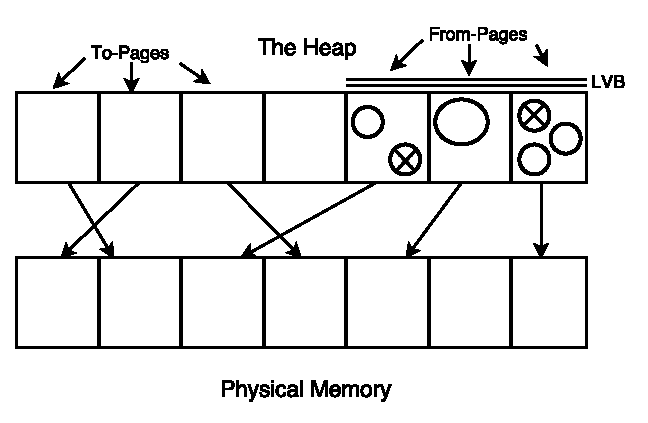
\psfig{file=c4_page_rough_2.pdf,width =3in}
\caption{In C4, memory is relocated
page-by-page. Dead objects are represented with X.
From-pages are protected from mutators by the LVB.}
\label{fig:c4Memory}
\end{figure}

%Contiguous virtual memory
%might not correspond to contiguous physical memory, which is out of scope for our discussion

C4 uses a read barrier called the \emph{Loaded Value Barrier} (LVB) to 
synchronize concurrent threads throughout the GC process~\cite{Tene:C4}. The LVB 
places \emph{invariants}, properties to be maintained, on each reference as it is loaded from memory.
One of the invariants relates to the tracing portion of the GC algorithm, so
it is not discussed here. The other invariant ensures
references loaded by a mutator during compaction must point to safely
accessible objects: objects that have already been moved.
If the invariant does not hold
when a reference is loaded, the barrier will trigger and correct
the situation as we discuss in the next Subsections.


\subsection{Concurrent Relocation}
\label{sec:c4Relocation}

The relocation phase of compaction in C4 occurs on a per-\emph{page}
basis, where a page is a fixed-length, contiguous block of virtual memory in the heap
backed by a contiguous block of physical storage~\cite{Tene:C4}.
To quickly empty pages, the most sparsely populated ones are relocated
first. In the case of Figure~\ref{fig:c4Memory}, the left-most 
\emph{from-page}, analogous to from-space, is relocated first as it has only one small object alive.
The object is copied to a \emph{to-page}, which is analogous to to-space.

From-pages are protected by the LVB as can be seen in Figure~\ref{fig:c4Memory}. 
LVB will trigger for mutator threads encountering a reference to an object
on a protected page. The mutator's subsequent behavior is:
\begin{itemize}
\item If the object is relocated already, find its new location
\item If the object is being relocated currently, wait until the GC thread is finished
\item If the object has not been relocated, move the object 
\end{itemize}
In all cases, the mutator cannot use the object until it is on a to-page.
Additionally, LVB has mutators correct the
references to avoid further barrier triggers on the same
reference.
Without mutator interference, GC threads will simply relocate the objects but
not remap references at this time. 

When all live objects are relocated from a from-page,
the C4 compactor will perform \emph{quick release}. 
The physical memory backing the page will be freed
once the last live object has been moved to a to-page. The objects have already 
been transferred to new pages, so the contents of the from-pages are no longer needed. The from-page 
will be in use as it still has references to it, but the physical memory can be recycled efficiently. 
In terms of Figure~\ref{fig:c4Memory}, the heap
memory seen on top is in use until after the remapping phase, but the physical memory below 
can be paired with a different virtual page and used immediately.


\subsection{Concurrent Remapping}
\label{sec:c4Remapping}

To maintain concurrency while updating all references to the now relocated
objects, the C4 compaction algorithm uses two techniques~\cite{Tene:C4}. The first is
\emph{lazy remapping}. With this, mutator
threads continue updating references as they trigger the LVB. In order for
the remapping phase to end, all live references must be updated.
This could go on indefinitely if lazy remapping alone is performed.

To finish remapping, a traversal of live references must be performed to
ensure all are updated; this is like the tracing traversal used to determine which
objects are garbage as discussed in Section 2.1. No physical resources are being held due
to quick release and lazy remapping does not severely impact mutator operations. 
As a result, the remapping traversal can wait until another GC cycle starts.
C4 will perform the remapping of one GC cycle during tracing
of the next cycle since both tasks traverse
the same references in memory. To
visualize how this works, examine Figure~\ref{fig:c4Cycle}. Upon remapping completion, 
all references to from-pages are now gone. Thus, the virtual addresses
are freed and reclamation of memory is now complete. 

\begin{figure}
\centering
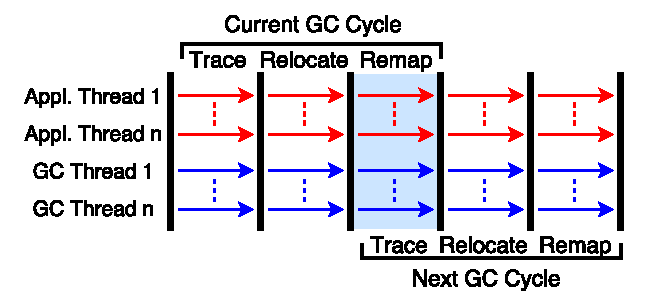
\psfig{file=c4Mapping_rough_figure_4.pdf,width =3in}
\caption{C4 GC cycle. Remapping and Tracing are rolled into one traversal.
(adapted from \cite{Tene:C4})}
\label{fig:c4Cycle}
\end{figure}


\subsection{C4 Results Summary}
\label{sec:c4Results}

% Tested primarily against also concurrent, but non-generational.

Experiments done with C4 were meant to show improvements
of using an algorithm that is simultaneously generational and concurrent~\cite{Tene:C4}.
C4 is tested against a modified, non-generational C4 algorithm as well as
two algorithms that do not perform concurrent compaction. 
All GC algorithms were tested on the same hardware; for specifications, see~\cite{Tene:C4}. 
The test exhibited live sets of objects on 
the heap consistently at a size of around 2.5 gigabytes (Gbs); the actual heap size was allowed 
to grow, indicating greater amounts of garbage on the heap. The applications were run long
enough to ensure multiple full-heap GC cycles ran and at least one
significant compaction event occurred.

The primary performance metric monitored was worst-case response times
of servers while experiencing the heap sizes
described, which provides a useful indicator of latency.
C4 maintained the smallest 
worst-case response times across the largest range of heap sizes.
The worst-case response times were usually in the range of 0.01-0.1 secs;
this is fast enough so an application user would not notice pauses. 
The non-generational version of C4 could also reach low worst-case response times,
but for a more limited range of heaps sizes. Standard
C4 sustained the times for heap sizes of 5-35 Gbs; the modified C4 could
only do so for heaps sizes of 15-35 Gbs. The non-concurrently compacting
collectors had multi-second worst-case response times for all heap sizes,
which would cause noticeable pauses for a users.


\section{The Collie Collector}
\label{sec:collie}

We now look at the concurrent compaction technique used by the single-threaded
Collie garbage collector described by Iynegar et al.~\cite{Iyengar:Collie}.
This is the same research group that worked on C4, so Collie utilizes modified 
versions of several techniques from C4, such as:
the tracing algorithm, the LVB, page-granularity compaction, and quick-release behavior.
Only the LVB is modified in significant ways as discussed below.
Like C4, the Collie
collector is designed with server environments and large heaps in mind.
However, it is not commercially available. 
Collie is implemented and tested in 
the same production-quality Azul JVM the Pauseless Garbage Collector is implemented 
in~\cite{Click:Pauseless}. 


\subsection{Transactional Memory}
\label{sec:collieTM}

The Collie's compaction algorithm sets itself apart due to use 
of a \emph{transactional memory} (TM) system as a concurrency control 
alternative to barriers~\cite{Iyengar:Collie}. TM systems allow
sections of code to function 
analogously to \emph{transactions} from database systems, 
which are a series of operations performed as one unit where 
they occur in an all-or-none manner.

For example, consider updating sale prices of items in a store; this requires
ensuring the store price matches the sale price advertised. 
When updating the prices for an item, both the
advertised price and the store price should be updated. Only updating the
advertised price could lead to irate customers, and only updating the
store price could lead to customers not knowing about the sale. A transaction
ensures an item's prices are unchanged if the update process 
is started and then aborted before completion. Additionally, customers cannot
see the prices mid-transaction; they only see the price from before the transaction began.

% Might be too much detail. Consider cutting later.
TM systems allow a series
of operations modifying memory to be placed in
a \emph{transactional procedure}, much like a database transaction.
The TM system monitors access of concurrent threads to \emph{transactional variables},
variables modified by a transactional procedure.
Concurrent threads will operate in parallel until they try to modify
the same transactional variable. How 
the conflict should resolve can be specified, but the general behavior would be for one transaction
to be aborted and the other allowed to continue.
When a transaction is completed, its changes are \emph{committed}; any changes 
made to memory by the transaction are finalized~\cite{wiki:transactional-memory}.

Each object on the heap has a \emph{referrer set}~\cite{Iyengar:Collie}. This is the precise set 
of all references pointing to the object. 
Referrer sets are stored as transactional variables since they are used by a transactional procedure 
(simply referred to as a transaction)
that relocates and remaps a single object.
An object must maintain a \emph{stable} referrer set throughout the GC process. That is,
its referrer set cannot be modified or expanded, which
ensures all of an object's references
are correctly remapped.



\subsection{The Collie Protocol}
\label{sec:collieProtocol}

After a tracing phase at the start of GC, heap compaction
happens during a \emph{transplantation phase}~\cite{Iyengar:Collie};
transplantation is a term meaning the combination of relocation and remapping.
Live objects and their referrer sets were determined during tracing. As mentioned, 
the operations for object transplantation are stored as a
transaction. Individual object transplantations are done only on objects 
that maintain stable referrer sets throughout the process.
An object is deemed \emph{non-individually transplantable} (NIT) if its transaction
is aborted or it fails to maintain a stable referrer set. 

Before performing the transactions to move individual objects, they
need to be checked for having stable referrer sets. To do this, threads' stacks
are checked for references to objects. Objects with references from stacks
will be marked NIT since mutators are using the objects, which could cause referrer set modifications.
This ensures GC does not interfere with mutator work.
The LVB-style read barrier receives its first new purpose here. When a thread attempts to load a reference,
and add it to its stack, the object the reference points to will be marked NIT as a mutator is using it.

The copying of an object actually occurs outside the transaction since any
mutator access of the object will trigger the LVB-style barrier,
rendering the object NIT. Thus, only remapping by updating the referrer set
is done in the transaction, which looks like:
\begin{enumerate}
\item Transaction is started
\item Object is checked to not have been marked NIT
\item All references are changed to point to the object's to-space location
\item Memory transaction is committed
\end{enumerate}
If a transaction fails or is interrupted, as detected by the TM system, the object is rendered NIT.


\subsection{Aborting Compactor}
\label{sec:collieAbortion}

After all individually transplantable objects are transplanted, we
are left with unmoved NIT objects.~\cite{Iyengar:Collie}.
However, compaction cannot terminate with objects in from-space.
The additions of a \emph{mirrored-to-space} and \emph{zero-copy transplantation} are necessary
to terminate compaction without disrupting mutators.

Mirrored-to-space is a virtual memory space corresponding to, and the same
size as, from-space. It is mapped to the same physical
memory as the corresponding from-space, as can be seen in Figure~\ref{fig:collieMirrored}. As mentioned, 
Collie uses page-granularity compaction like C4. From-space is used here 
to refer to the set of from-pages with NIT objects. For compaction 
termination purposes, mirrored-to-space is logically considered a part of to-space.

Zero-copy transplantation gets the compactor to believe it has finished a cycle.
Mirrored-to-space holds the same objects in physical memory as from-space.
Thus, if references
are remapped to mirrored-to-space from from-space,
the objects appear to be relocated without physically moving. This technique
is zero-copy transplantation. In Figure~\ref{fig:collieMirrored},
all references are to from-space for NIT objects. After zero-copy transplantation, they
point to mirrored-to-space.

Zero-copy transplantation
is performed on all NIT objects. The LVB-style barrier receives a second purpose here. As mutators
access references to NIT objects before they are updated to mirrored-to-space, 
the barrier will cause the mutators to correct the references before using the object. Also like
C4, entirely finishing zero-copy transplantation, which is just remapping, is rolled
up into the next GC cycle's tracing phase. In the end, NIT objects are not actually compacted;
for this reason, Collie is said to have an \emph{aborting} compactor. It will
cease moving objects to allow mutator threads to continue working uninterrupted.

\begin{figure}
\centering
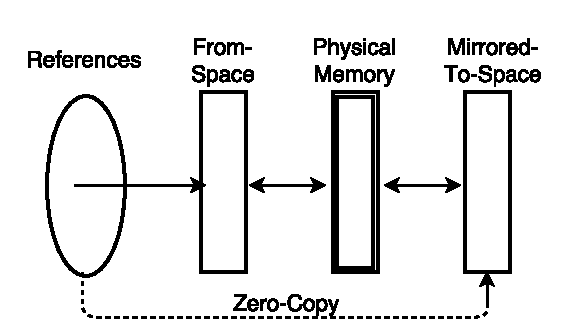
\psfig{file=collie_mirrored_rough.pdf,width =3in}
\caption{Mirrored-to-space and zero-copy transplantation in Collie}
\label{fig:collieMirrored}
\end{figure}


\subsection{Collie Results Summary}
\label{sec:collieResults}

% Tested primarily against Another concurrent that is also modified to run on a single thread.

The main goal of the Collie collector is to decrease latency
during compaction~\cite{Iyengar:Collie}. The Collie was tested 
against a modified variant of the Pauseless Garbage Collector~\cite{Click:Pauseless}.
Accordingly, both collectors were implemented within the same JVM. For exact
testing specifications, refer to~\cite{Iyengar:Collie}. The Collie
utilizes several aspects of C4, which in turn builds upon the Pauseless
collector. This provides an effective comparison to see how 
use of transactional memory and an aborting compactor affect application performance. 

To examine latency, \emph{minimum mutator utilization} (MMU) is measured.
MMU is the minimum percentage of mutators being utilized over a period of time. Ideally,
MMU would always be at 100\% so all mutators are being used. 
MMUs were taken from various time periods during which
compaction was running and was compared between the two algorithms. Comparisons were done
with a 128 megabyte (Mb) heap and a 512 Mb heap. For all time windows, the Collie compactor
had higher MMUs than Pauseless. Collie did not go below a 70\% mutator utilization 
level whereas Pauseless averaged between 40\% and 70\%. 
This shows the aborting nature of Collie
lends itself to ensuring mutator response time, and thus decreasing latency, 
despite potentially limiting the amount of memory compacted.


\section{Field Pinning Protocol}
\label{sec:fpp}

Last, we examine concurrent compaction in GC through a Field Pinning
Protocol (FPP), designed by \"{O}sterlund and L\"{o}we~\cite{Osterlund:FPP}.
FPP describes a barrier-free process for performing the relocation aspect
of concurrent compaction. The remapping phase and other portions
of GC are left up to the host garbage collector. FPP is compliant with the Java Native Interface
to allow for integration into a JVM. For purposes of testing, FPP 
is implemented within the Garbage-First GC algorithm in the HotSpot JVM 
of OpenJDK 9~\cite{Detlefs:G1}, which lacks concurrent relocation.


\subsection{Hazard Pointers}
\label{sec:fppHazard}

The key component driving FPP is the \emph{hazard pointer} (HP)~\cite{Osterlund:FPP}. 
In FPP, all mutator threads contain a list of HPs.
The HPs point to objects in memory a thread is accessing, or \emph{pin} them.
When a thread finishes using an object, it drops the HP.
So long as an object
is pinned by a mutator, it cannot be relocated as it is still in use. Once all threads have
unpinned the object, it can safely be relocated.
When discussing the theoretical construction of the algorithm, a granularity of pinning 
individual fields is used, thus the name \emph{Field} Pinning Protocol. 

% Changed from original example using cake. May want to change back depending
% on reader feedback. Cake at a party.
While it is explained in more detail below, an example of how HPs 
work on a high-level is useful. Imagine a pot of coffee at work. Anyone 
wanting coffee must make it known to others by having a cup, otherwise the 
coffee is liable to be moved to another break room. The people are effectively pinning the coffee.
Once everyone has had their share of caffeine, it should be moved. This can
be done safely when no one has cups any longer, so the coffee is not pinned.

% Took out from this example that last person to discard the cup will be responsible.
% Did so to be able to build on the example.


\subsection{Collaborative Copying and Blame}
\label{sec:fppCopy}

HPs prevent premature relocation of objects by serving as a distributed
counter. Threads cannot relocate objects with a HP count greater than zero.
A mutator thread \emph{impedes} a copying thread if
its HP prevents the copying.
The impeding thread is \emph{blamed} for the 
interruption~\cite{Osterlund:FPP}; it becomes responsible for ensuring 
the object is relocated. GC threads cannot receive blame as they will not impede
copy attempts.

The process followed by mutator threads during the relocation phase when 
accessing an object is as follows:
\begin{enumerate}
\item Pin the object by adding a HP
\item Determine whether the object has already been copied
\item Mutate/use the object. Since the object is pinned, the thread can 
do so without worry
\item Unpin the object when no longer needed
\item If the thread was blamed due to impeding another thread's copy attempt, 
attempt to copy the object:
\begin{enumerate}
\item Check other threads for HPs before copying. If HPs found,
blame all the threads and move along
\item Proceed to copy the object with further pins still impeding the copy
\end{enumerate}
\end{enumerate}
Mutators will continually bounce blame around until
no threads have the object pinned. At this time, the last thread
to attempt to copy the object will succeed.

Reconsider the coffee example. Suppose
someone is in charge of moving the coffee to the other room.
Much like how a GC thread must relocate objects. They
can try, but others could still have cups and want more coffee.
The interrupted person has other tasks they could be doing, so they tell
everyone with a cup to move the coffee when finished drinking it;
they blame the others for not finishing the task and make them responsible
for it. When those blamed finish their coffee, they will try to
move it as well. If interrupted by others with coffee cups, HPs, they
pass the blame along. This continues until a last person finishes 
their coffee.

At the start of FPP relocation, GC threads will attempt to copy
objects marked for relocation. At this time, blaming is 
disabled. 
After the first round of attempting to copy objects, the GC threads
will again try to copy the remaining objects. If a mutator 
thread impedes the copy attempt this time, it will be blamed.
Blame continues to be passed until the objects are relocated. 

It is possible for an
object not to move because it is continually pinned. How this terminates 
depends on the host GC algorithm used. When using the Garbage-First (G1) algorithm,
this process goes until all objects are moved or another GC cycle starts.
If objects have not relocated when another cycle begins, they are automatically
marked for relocation again. Allowing mutators to continue passing blame works
in G1 because, like C4 and Collie, the algorithm will roll up remapping into the next
GC cycle's tracing phase. Possible alternatives include setting a max number of impediments
or setting a timer.


\subsection{FPP Results Summary}
\label{sec:fppResults}

% Tested against a concurrent collector that does NOT have concurrent compaction.

As mentioned, FPP was implemented in the G1 garbage collector for testing purposes~\cite{Osterlund:FPP}. 
Appropriately, the modified G1 collector utilizing FPP for relocation is tested against the
unmodified G1 collector. This was tested in a MacBook Pro; for the 
hardware details, see~\cite{Osterlund:FPP}. We focus on the tests comparing
latency of the two garbage collectors. For other tests performed and their results, see~\cite{Osterlund:FPP}.

For latency, the h2 benchmark from DaCapo is used~\cite{Blackburn:DaCapo}.
The benchmark was chosen due to being memory intensive,
which makes latency issues apparent.
Latency is measured using the jHiccup tool developed by Azul Systems.
Compared to its host garbage collector, G1 with FPP improved latency at all time
intervals examined. On average, latency was improved by around 50\%; application
pause times were about half as long. Latency was also shown to mostly be caused by 
host garbage collector activities such as tracing and remapping.


\section{Conclusions}
\label{sec:conclusions}

We have examined three concurrent compaction techniques that are 
effective in reducing latency of garbage collectors.
The garbage collectors implemented in were tested for latency in
different manners and against various algorithms, so it is difficult to 
compare them to one another. Direct comparisons are made even more difficult since the
algorithms were not all designed for the same environment.

The algorithms we have looked at achieved concurrency while maintaining low latency in various
ways. C4 and Collie both use read barriers differently. C4 
uses a barrier to control mutator behavior, and Collie uses one to allow mutators to
work without interruption. FPP takes a wholly different approach by focusing on 
performing relocation alone without any barriers; it avoids standard synchronization methods by using HPs
and thread collaboration instead.
Regardless of approach, compaction is necessary for efficient GC with growing heaps and
increasing environmental demands. Ultimately,
the approach for compaction used will depend on its intended environment.


\section*{Acknowledgments}
\label{sec:acknowledgments}

% To be updated as time goes on.

Thank you Elena Machkasova and Jeff Lindblom for the great advice and feedback.
Thank you Jeremy Eberhardt for infinite words of wisdom throughout.


% The following two commands are all you need in the
% initial runs of your .tex file to
% produce the bibliography for the citations in your paper.
\bibliographystyle{abbrv}
% sample_paper.bib is the name of the BibTex file containing the
% bibliography entries. Note that you *don't* include the .bib ending here.
\bibliography{sample_paper}  
% You must have a proper ".bib" file
%  and remember to run:
% latex bibtex latex latex
% to resolve all references

\end{document}
